\subsubsection{Giới thiệu bộ dữ liệu}
    \paragraph{Nguồn dữ liệu}
    \leavevmode

    Bộ dữ liệu được thu thập bởi Rakesh Kapilavayi, viện công nghệ thông tin Vishnu, Ấn Độ, thông qua Google Forms trong dự án nghiên cứu các đặc điểm tính cách và xu hướng hành vi ở sinh viên của anh ta. 

    \paragraph{Mô tả dữ liệu}
    \leavevmode

    Đây là bộ dữ liệu chứa thông tin khảo sát các sinh viên, mỗi dòng là thông tin liên quan đến đặc điểm hành vi, tính cách do người tham gia khảo sát trả lời. 

    Ví dụ một phần dữ liệu:

    \begin{table}[htbp]
    \centering
    \caption{Một phần bảng dữ liệu Behavior dataset}
    \label{tab:stat-behavior-exp}
        \begin{tabular}{|p{1.5cm}|p{1.5cm}|p{2cm}|p{1.5cm}|p{2cm}|p{2cm}|p{1.75cm}|p{2cm}|}
        \hline
        Time spent Alone & Stage fear & Social event attendance & Going outside & Drained after socializing & Friends circle size & Post frequency & Personality \\
        \hline
        4 & No & 4 & 6 & No & 13 & 5 & Extrovert \\
        \hline
        9 & Yes & 0 & 0 & Yes & 0 & 3 & Introvert \\
        \hline
        9 & Yes & 1 & 2 & Yes & 5 & 2 & Introvert \\
        \hline
        0 & No & 6 & 7 & No & 14 & 8 & Extrovert \\
        \hline
        ... & ... & ... & ... & ... & ... & ... & ... \\
        \hline
        \end{tabular}

    \end{table}

    Bộ dữ liệu có 2,900 dòng, bao gồm 8 cột như sau:

    \begin{itemize}
        \item Kiểu dữ liệu: \textbf{Qualitative} 

        \begin{enumerate}
            \item \textbf{Stage\_fear}: Sợ sân khấu/đứng trước đám đông (Yes/No)

            \item \textbf{Drained\_after\_socializing}: Cảm thấy mệt mỏi sau khi xã giao (Yes/No)

            \item \textbf{Personality}: Tính cách (Extrovert, Introvert)
            
        \end{enumerate}

        \item Kiểu dữ liệu: \textbf{Quantitative} 
        \begin{itemize}
            \item \textbf{Discrete}:

                \begin{enumerate}[resume]
                    \item \textbf{Time\_spent\_Alone}: Thời gian một mình mỗi ngày (0–11)

                    \item \textbf{Social\_event\_attendance}: Mức độ tham gia sự kiện xã hội (0–10, người tham gia tự đánh giá từ 0, rất ít, đến 10, rất nhiều)

                    \item \textbf{Going\_outside}: Mức độ ra ngoài (0–7, người tham gia tự đánh giá từ 0, ít khi, đến 7, thường xuyên)

                    \item \textbf{Friends\_circle\_size}: Số lượng bạn gần gũi (0-15)

                    \item \textbf{Post\_frequency}: Mức độ đăng bài lên mạng xã hội (ít khi 0–10 thường xuyên)

                \end{enumerate}
        \end{itemize}
     
     \end{itemize}

\subsubsection{Các nghiên cứu liên quan}

    Tác giả Rakesh Kapilavayi \cite{kapilavayi} áp dụng quy trình xử lý dữ liệu làm sạch dữ liệu, phân tích mối quan hệ giữa các đặc trưng đến lựa chọn mô hình học máy phù hợp như Random Forest, XGBoost và SVM. Kết quả thu được không chỉ chứng minh hiệu quả của các thuật toán học máy trong lĩnh vực phân tích nhân cách mà còn mở ra hướng tiếp cận mới trong phát triển các hệ thống hỗ trợ đánh giá tâm lý - nhân sự, giáo dục cá nhân hóa hoặc các nền tảng tương tác người dùng thông minh.

    Nghiên cứu \cite{article_tab_3}tập trung vào việc đánh giá độ tin cậy của bộ cơ sở dữ liệu sàng lọc rối loạn phổ tự kỷ (ASD) trẻ em trên kho dữ liệu UCI bằng cách áp dụng các thuật toán học máy. Các nhà nghiên cứu đã sử dụng bộ dữ liệu sàng lọc ASD trẻ em từ kho dữ liệu UCI, bao gồm 292 trường hợp, và một bộ dữ liệu kiểm nghiệm thực tế gồm 18 trường hợp do các chuyên gia thu thập. Quá trình tiền xử lý dữ liệu bao gồm xóa các trường hợp thiếu dữ liệu và lựa chọn 10 đặc trưng liên quan nhất bằng phương pháp Chi Square. Nghiên cứu đã xây dựng mô hình dự đoán bằng cách khảo sát bảy thuật toán học máy: SVM, Random Forest, Decision Trees, Logistic Regression, K-Nearest-Neighbors, Naïve Bayes, và Multi Layer Perceptron (MLP), với kỹ thuật xác thực chéo 10 lần (10-fold cross-validation) để nâng cao chất lượng mô hình. Kết quả thử nghiệm cho thấy tất cả bảy thuật toán đều cho kết quả phân loại cao, phù hợp với các nghiên cứu trước đó. Đặc biệt, các thuật toán Random Forest, SVM, Logistic Regression, KNN và MLP đã đạt tỷ lệ dự đoán đúng 100\% trên bộ dữ liệu thực tế. Từ những kết quả này, nghiên cứu kết luận rằng bộ dữ liệu phân loại rối loạn phổ tự kỷ trẻ em trên kho dữ liệu UCI là đáng tin cậy và đề xuất sử dụng mô hình thuật toán SVM để phát triển ứng dụng sàng lọc ASD trẻ em.

\subsubsection{Phân tích dữ liệu}

    \paragraph{Thống kê dữ liệu}
        \leavevmode

     Bảng \ref{tab:stat-behavior} thể hiện các thông số thống kê trên một số đặc trưng của bộ dữ liệu.
     
    \begin{table}[htbp]
    \centering
    \caption{ Thống kê dữ liệu một số đặc trưng dữ liệu Behavior dataset}
    \label{tab:stat-behavior}
    \begin{tabular}{|p{2cm}|p{2cm}|p{2cm}|p{2cm}|p{2cm}|p{2cm}|}
        \hline
        & Post frequency & Friends circle size & Going outside & Social event attendance & Time spent Alone \\
        \hline
        Mean & 3.5647 & 6.2689 & 3 & 3.9634 & 4.5058 \\
        \hline
        Min & 0 & 0 & 0 & 0 & 0 \\
        \hline
        Q1 & 1 & 3 & 1 & 2 & 2 \\
        \hline
        Median & 3 & 5 & 3 & 3.9634 & 4 \\
        \hline
        Q3 & 6 & 10 & 5 & 6 & 7 \\
        \hline
        Max & 10 & 15 & 7 & 10 & 11 \\
        \hline
        Mode & 2 & 5 & 0 & 2 & 0 \\
        \hline
        Var & 8.3728 & 17.9127 & 4.9355 & 8.2519 & 11.8417 \\
        \hline
        SD & 2.8936 & 4.2323 & 2.2216 & 2.8726 & 3.4412 \\
        \hline
        CV & 0.8117 & 0.6751 & 0.7405 & 0.7248 & 0.7637 \\
        \hline
        IQR & 5 & 7 & 4 & 4 & 5 \\
        \hline
    \end{tabular}
    \end{table}

    Từ Bảng \ref{tab:stat-behavior}, ta có thể rút ra một số nhận xét:
    
    \begin{itemize}
    \item Post frequency: Trung bình là 3.56 bài, trung vị là 3 và mode là 2, cho thấy tần suất đăng bài khá đồng đều, phần lớn người dùng đăng bài ở mức thấp đến trung bình. Độ lệch chuẩn 2.89 tương đối cao so với trung bình, thể hiện sự phân tán khá lớn, có thể do một số ít người đăng bài rất thường xuyên (max = 10), trong khi một số khác không đăng gì (min = 0)
    
    \item Friends circle size: Giá trị trung bình 6.27 và trung vị là 5. Tuy nhiên, giá trị max = 15 và SD = 4.23 phản ánh sự phân tán cao, có thể do một số người có mạng lưới bạn rất rộng trong khi số khác thì không. Mode = 5 phù hợp với median, cho thấy có tính tập trung cao quanh trung vị.
    
    \item Going outside: Trung bình và trung vị đều là 3, cho thấy mức độ ra ngoài vừa phải là phổ biến. Mode = 0 cho thấy đa số không tích ra ngoài. Độ lệch chuẩn 2.22 tương đối lớn so với trung bình.
    
    \item Social event attendance: Trung bình, trung vị bằng 3.96 và mode = 2. SD = 2.87 và IQR = 4 cho thấy dữ liệu không phân bố rộng.
    
    \item Time spent Alone: Trung bình là 4.51, trung vị là 4, và mode = 0, cho thấy có nhiều người dành thời gian một mình mỗi ở mức trung bình đến cao.
    
    \end{itemize}

    \paragraph{Trực quan hóa dữ liệu}
    \leavevmode

    \begin{figure}[htp]
        \centering
        \begin{subfigure}{0.33\textwidth}
            \centering
            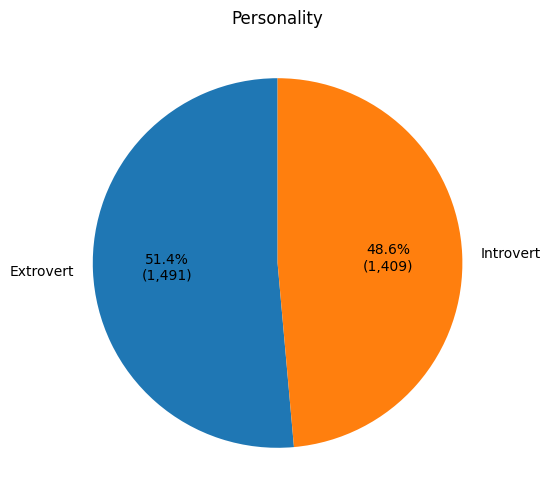
\includegraphics[width=\textwidth]{images/Table_behavior_personality.png}
            \caption{Tính cách}
            \label{fig:Table_behavior_personality}
        \end{subfigure}
        \vspace{0.5cm}
        \begin{subfigure}{0.3\textwidth}
            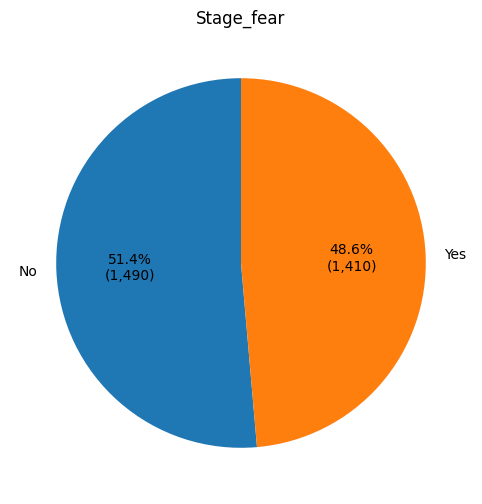
\includegraphics[width=\textwidth]{images/Table_behavior_stagefear.png}
            \caption{Sợ sân khấu/đám đông}
            \label{fig:Table_behavior_stagefear}
        \end{subfigure}
        \hfill
        \begin{subfigure}{0.3\textwidth}
            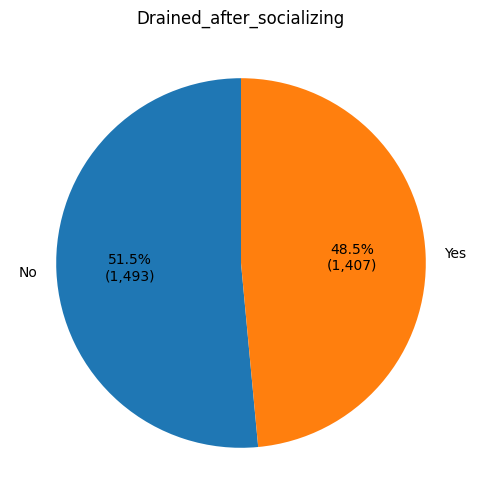
\includegraphics[width=\textwidth]{images/Table_behavior_drain.png}
            \caption{Mệt mỏi sau khi xã giao}
            \label{fig:Table_behavior_drain}
        \end{subfigure}
        \caption{Phân phối nhãn các cột qualitative}
        \label{fig:Table_behavior_qualitative}
    \end{figure}

    \FloatBarrier

    Các biểu đồ pie\ref{fig:Table_behavior_qualitative} cho thấy sự phân phối dữ liệu giữa các nhãn thuộc các cột 'Personality', 'Stage\_fear', 'Drained\_after\_socializing' là gần như cân bằng.

    \begin{figure}[htp]
        \centering
        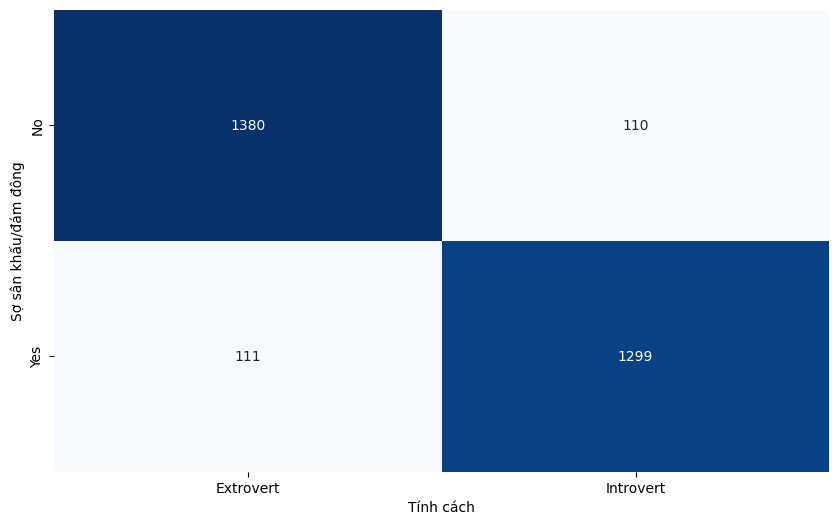
\includegraphics[width=0.8\textwidth]{images/Table_behavior_stagefear_personality.png}
        \caption{Tương quan 'Stage\_fear' và 'Personality'}
        \label{fig:Table_behavior_stagefear_personality}
    \end{figure}

    \FloatBarrier

    Biểu đồ heatmap \ref{fig:Table_behavior_stagefear_personality} cho thấy tương quan mạnh giữa 'Stage\_fear' và 'Personality'. Đa phần những người không có tính 'Sợ đám đông' đa phần thuộc nhóm tính cách 'Extrovert' và ngược lại.

    \begin{figure}[htp]
        \centering
        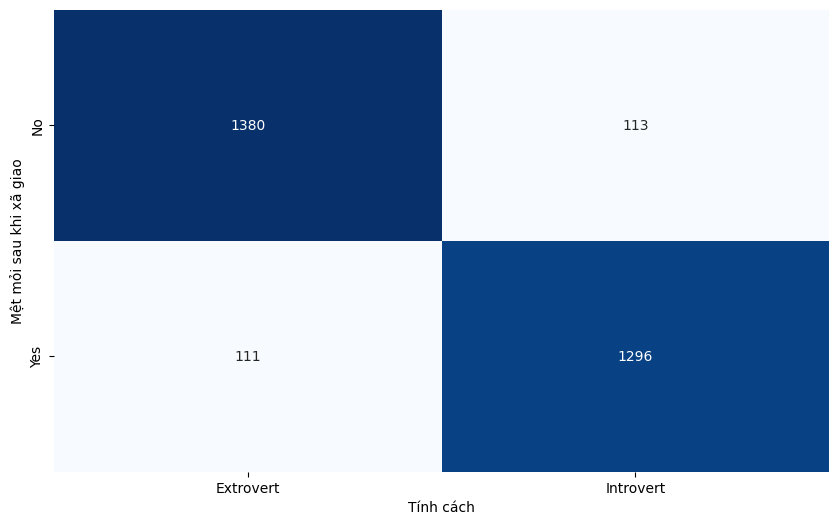
\includegraphics[width=0.8\textwidth]{images/Table_behavior_drain_personality.png}
        \caption{Tương quan 'Drained\_after\_socializing' và 'Personality'}
        \label{fig:Table_behavior_drain_personality}
    \end{figure}

    \FloatBarrier

    Biểu đồ heatmap \ref{fig:Table_behavior_drain_personality} cho thấy tương quan mạnh giữa 'Drained\_after\_socializing' và 'Personality'. Đa phần những người không bị 'Mệt mỏi sau khi xã giao' đa phần thuộc nhóm tính cách 'Extrovert' và ngược lại.

    \begin{figure}[htp]
        \centering
        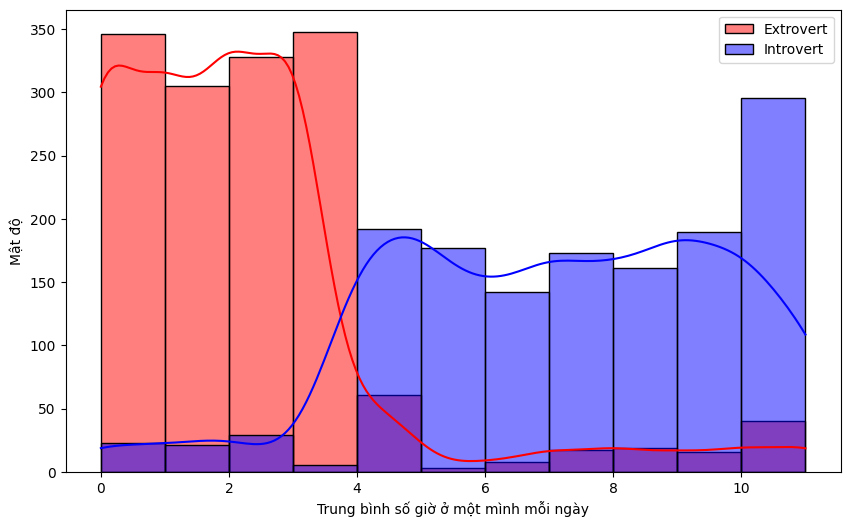
\includegraphics[width=0.9\textwidth]{images/Table_behavior_timealone_personality.png}
        \caption{Phân phối trung bình số giờ ở một mình theo tính cách}
        \label{fig:Table_behavior_timealone_personality}
    \end{figure}
    \FloatBarrier

    Biểu đồ \ref{fig:Table_behavior_timealone_personality} thể hiện sự phân bố thời gian trung bình mỗi ngày một người ở một mình phân loại theo tính cách. Biểu đồ này phản ánh sự khác biệt rõ rệt trong hành vi giữa hai nhóm tính cách. Người hướng ngoại (Extrovert) chủ yếu dành từ 0 đến 4 giờ mỗi ngày để ở một mình. Đường cong mật độ màu đỏ cho thấy xu hướng giảm mạnh sau mốc 4 giờ, cho thấy rất ít người hướng ngoại dành quá nhiều thời gian ở một mình. Ngược lại, người hướng nội (Introvert) lại có xu hướng dành nhiều thời gian hơn ở một mình. Phần lớn nằm trong khoảng từ 5 giờ trở lên mỗi ngày.

    \begin{figure}[htp]
        \centering
        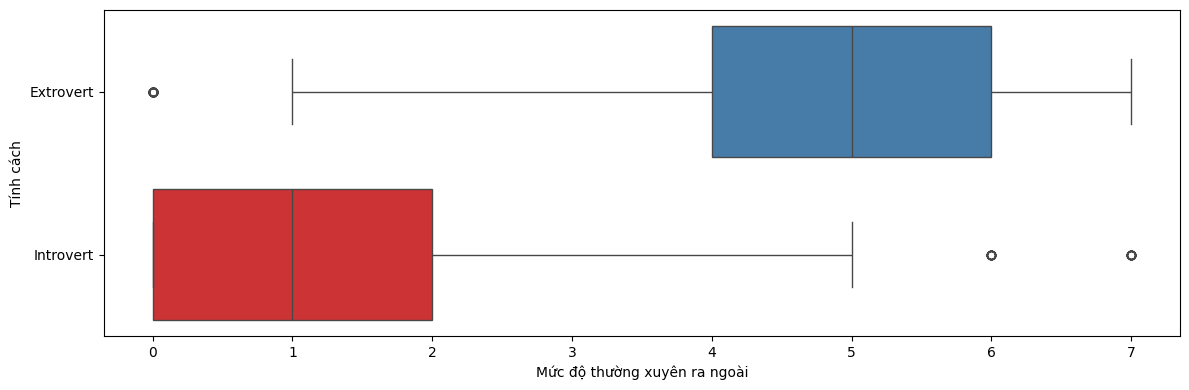
\includegraphics[width=0.9\textwidth]{images/Table_behavior_goingout_personality.png}
        \caption{Phân phối trung bình số giờ ở một mình theo tính cách}
        \label{fig:Table_behavior_goingout_personality}
    \end{figure}
    \FloatBarrier

    Biểu đồ \ref{fig:Table_behavior_goingout_personality} phản ánh hai tính cách có hướng hành vi đặc trưng riêng. Người hướng ngoại có mức độ ra ngoài cao hơn rõ rệt, với phần lớn giá trị nằm ở khoản trên 4. Trung vị của nhóm này là 5, cho thấy họ thường xuyên tham gia vào các hoạt động bên ngoài. Trong khi đó, người hướng nội có mức độ ra ngoài thấp hơn đáng kể, với trung vị 1 và phần lớn giá trị tập trung dưới 2 kèm một vài ngoại lệ

    \begin{figure}[htp]
        \centering
        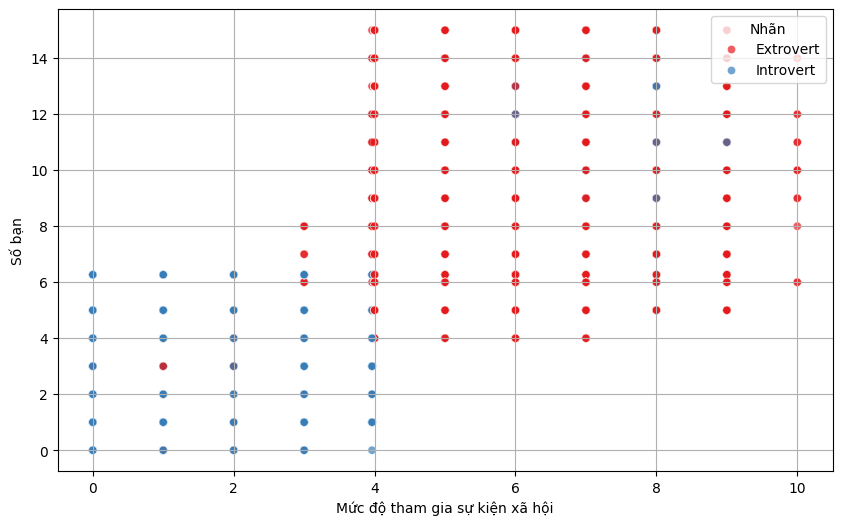
\includegraphics[width=0.9\textwidth]{images/Table_behavior_event_friend_personality.png}
        \caption{Tương quan 'Social\_event\_attendance' và 'Friends\_circle\_size' theo nhãn 'Personality'}
        \label{fig:Table_behavior_event_friend_personality}
    \end{figure}
    \FloatBarrier

    Biểu đồ \ref{fig:Table_behavior_event_friend_personality} cho thấy 'Social\_event\_attendance' và 'Friends\_circle\_size' có tương quan thuận. Người có 'Số bạn' cao thì 'Mức độ tham gia sự kiện xã hội' cũng tăng theo và ngược lại. Và biểu đồ cũng cho thấy các điểm có thể phân ra thành 2 vùng rõ rệt cho hai nhãn tính cách. Với 'Số bạn' trên 6 và 'Mức độ tham gia sự kiện' trên 5 tạo thành vùng tính cách hướng ngoại, còn lại là tính cách hướng nội, với một số điểm ngoại lệ.

\subsubsection{Mô hình hóa dữ liệu}
    \paragraph{Cấu hình cài đặt} 
    \leavevmode

    Các mô hình sử dụng:

    \begin{itemize}
        \item \textbf{Logistic Classification}: 

            \begin{lstlisting}[language=Python]
                LogisticRegressionCV(
                    max_iter=max_iter,
                    Cs=cs,
                )
            \end{lstlisting}

            khoảng hypertune tham số

            \begin{lstlisting}[language=Python]
                list_max_iter = [10, 20, 30, 40, 50, 100, 200, 300, 500]
                list_cs = [1,2,3,4,5,8,10]
            \end{lstlisting}.

        \item \textbf{Random Forest Classifier}:

            \begin{lstlisting}[language=Python]
                RandomForestClassifier(
                    max_depth=max_depth,
                    n_estimators=n_estimators,
                    min_samples_leaf=min_samples_leaf,
                )
            \end{lstlisting}

            khoảng hypertune tham số

            \begin{lstlisting}[language=Python]
                list_max_depth = [2, 3, 5, 10]
                list_n_estimators = [50, 100, 150, 200]
                list_min_samples_leaf = [3, 5, 10, 20]
            \end{lstlisting}.

        \item \textbf{XGBoost Classifier}:
            \begin{lstlisting}[language=Python]
                XGBClassifier(
                    max_depth=max_depth,
                    n_estimators=n_estimators,
                    reg_lambda=reg_lambda,
                    learning_rate=lr,
                    reg_alpha=alpha,
                )
            \end{lstlisting}

            khoảng hypertune tham số

            \begin{lstlisting}[language=Python]
                list_max_depth = [ 6, 7, 8, 9]
                list_lambda = [0.5, 1, 2]
                list_learning_rate = [1, 0.8, 0.5, 0.25]
                list_n_estimators = [50, 100, 150, 200]
                list_alpha = [0.5, 1, 2]
            \end{lstlisting}.
        
    \end{itemize}

    Thuật toán data transform sử dụng: Standard Scaler.

    Chia tập dữ liệu huấn luyện: Cross-validation 5 folds.

    \paragraph{Phân lớp tính cách 'Personality'}
    \leavevmode

    Chọn các đặc trưng huấn luyện: 'Stage\_fear', 'Drained\_after\_socializing', 'Time\_spent\_Alone', 'Social\_event\_attendance', 'Going\_outside', 'Friends\_circle\_size', 'Post\_frequency'

    Kết quả:
    \begin{itemize}
        \item \textbf{Logistic Classification}: 
        
            Mô hình tốt nhất:
            \begin{itemize}
                \item max\_iter: 10
                \item cs: 1
            \end{itemize}

            \begin{table}[htbp]
            \centering
            \caption{Kết quả Logistic Classification - Phân lớp tính cách}
            \label{tab:Behavior-personality-LogCV}
            \begin{tabular}{lrrrrrr}
                \hline
                & train\_acc & test\_acc & test\_recall & test\_precision & test\_f1 & test\_roc\_auc \\
                \hline
                mean & 0.934483 & 0.934483 & 0.925555 & 0.945973 & 0.935549 & 0.909680 \\
                std & 0.002859 & 0.011437 & 0.018584 & 0.012504 & 0.011448 & 0.021048 \\
                min & 0.930172 & 0.922414 & 0.909396 & 0.929293 & 0.923339 & 0.888679 \\
                max & 0.937500 & 0.951724 & 0.956376 & 0.961131 & 0.953177 & 0.938883 \\
                \hline
            \end{tabular}
            \end{table}
  
            
            \FloatBarrier
            
        \item \textbf{Random Forest Classifier}:

            Mô hình tốt nhất:
            \begin{itemize}
                \item max\_depth: 2
                \item n\_estimators: 50
                \item min\_samples\_leaf: 3
            \end{itemize}

            \begin{table}[htbp]
                \centering
                \caption{Kết quả Random Forest Classifier - Phân lớp tính cách}
                \label{tab:Behavior-personality-RF}
                \begin{tabular}{lrrrrrr}
                    \hline
                     & train\_acc & test\_acc & test\_recall & test\_precision & test\_f1 & test\_roc\_auc \\
                    \hline
                    mean & 0.934483 & 0.934483 & 0.925555 & 0.945973 & 0.935549 & 0.959291 \\
                    std & 0.002859 & 0.011437 & 0.018584 & 0.012504 & 0.011448 & 0.008782 \\
                    min & 0.930172 & 0.922414 & 0.909396 & 0.929293 & 0.923339 & 0.945732 \\
                    max & 0.937500 & 0.951724 & 0.956376 & 0.961131 & 0.953177 & 0.968442 \\
                    \hline
                \end{tabular}
            \end{table}
            
            \FloatBarrier

        \item \textbf{XGBoost Classifier}:
        
            Mô hình tốt nhất:
            \begin{itemize}
                \item max\_depth: 6
                \item n\_estimators: 100
                \item reg\_lambda: 0.5
                \item reg\_alpha: 2
                \item learning\_rate: 0.25
            \end{itemize}

            \begin{table}[htbp]
                \centering
                \caption{Kết quả XGBoost Classifier - Phân lớp tích cách}
                \label{tab:Behavior-personality-XGBC}
                \begin{tabular}{lrrrrrr}
                \hline
                 & train\_acc & test\_acc & test\_recall & test\_precision & test\_f1 & test\_roc\_auc \\
                \hline
                mean & 0.936897 & 0.933103 & 0.923539 & 0.945228 & 0.934151 & 0.962129 \\
                std & 0.001869 & 0.011200 & 0.018143 & 0.013075 & 0.011241 & 0.009516 \\
                min & 0.934914 & 0.920690 & 0.906040 & 0.928814 & 0.921502 & 0.947868 \\
                max & 0.939224 & 0.946552 & 0.953020 & 0.961131 & 0.948247 & 0.972851 \\
                \hline
                \end{tabular}
            \end{table}

            \FloatBarrier
    \end{itemize}

    So sách các mô hình:

    \begin{table}[htbp]
        \centering
        \caption{So sánh kết quả các mô hình (và nghiên cứu liên quan) - Phân lớp tính cách}
        \label{tab:Behavior-personality-compare}
        \begin{tabular}{|p{2cm}|p{2cm}|p{2cm}|p{2cm}|p{2cm}|p{2cm}|}
            \hline
             Model & Mean Test Accuracy & Mean F1 & Mean Recall & Mean Precision & Mean ROC AUC \\
            \hline
            Logistic Regression & \textbf{0.934483} & \textbf{0.935549} & \textbf{0.925555} & \textbf{0.945973} & 0.909680 \\
            \hline
             Random Forest & \textbf{0.934483} & \textbf{0.935549} & \textbf{0.925555} & \textbf{0.945973} & 0.959291 \\
            \hline
             XGBoost & 0.933103 & 0.934151 & 0.923539 & 0.945228 & \textbf{0.962129} \\
            \hline
             Rakesh Kapilavayi \cite{kapilavayi} &  & 0.92 & 0.94 & 0.94 & 0.95 \\
            \hline
        \end{tabular}
    \end{table}

    \FloatBarrier

    Xét tổng thể, cả ba mô hình đều cho kết quả rất tương đồng, với độ chính xác, F1, Recall và Precision gần như giống hệt nhau. Logistic Regression và Random Forest có cùng kết quả trên toàn bộ các chỉ số chính ngoại trừ ROC AUC thì Random Forest cao hơn. XGBoost có chỉ thấp hơn rất ít so với hai mô hình còn lại, nhưng lại đạt giá trị ROC AUC cao nhất (0.962129), cho thấy khả năng phân biệt giữa các lớp tốt hơn.

    So với thực hiện trước đó của tác giả \cite{kapilavayi}, các mô hình đều cho kết quả tốt hơn.

    \FloatBarrier


    \paragraph{Phân lớp 'Drained after socializing'}
    \leavevmode

    Chọn các đặc trưng huấn luyện: 'Stage\_fear', 'Time\_spent\_Alone', 'Social\_event\_attendance', 'Going\_outside', 'Friends\_circle\_size', 'Post\_frequency'

    Kết quả:
    \begin{itemize}
        \item \textbf{Logistic Classification}: 
        
            Mô hình tốt nhất:
            \begin{itemize}
                \item max\_iter: 10
                \item cs: 1
            \end{itemize}

            \begin{table}[htbp]
            \centering
            \caption{Kết quả Logistic Classification - Phân lớp 'Drained after socializing'}
            \label{tab:Behavior-drain-LogCV}
            \begin{tabular}{lrrrrrr}
                \hline
                & train\_acc & test\_acc & test\_recall & test\_precision & test\_f1 & test\_roc\_auc \\
                \hline
                mean & 0.988276 & 0.988276 & 1.000000 & 0.976432 & 0.988068 & 0.989695 \\
                std & 0.000771 & 0.003084 & 0.000000 & 0.006101 & 0.003116 & 0.003183 \\
                min & 0.987069 & 0.986207 & 1.000000 & 0.972318 & 0.985965 & 0.985479 \\
                max & 0.988793 & 0.993103 & 1.000000 & 0.986014 & 0.992958 & 0.993882 \\
                \hline
            \end{tabular}
            \end{table}
  
            
            \FloatBarrier
            
        \item \textbf{Random Forest Classifier}:

            Mô hình tốt nhất:
            \begin{itemize}
                \item max\_depth: 2
                \item n\_estimators: 50
                \item min\_samples\_leaf: 3
            \end{itemize}

            \begin{table}[htbp]
                \centering
                \caption{Kết quả Random Forest Classifier - Phân lớp 'Drained after socializing'}
                \label{tab:Behavior-drain-RF}
                \begin{tabular}{lrrrrrr}
                    \hline
                     & train\_acc & test\_acc & test\_recall & test\_precision & test\_f1 & test\_roc\_auc \\
                    \hline
                    mean & 0.988276 & 0.988276 & 1.000000 & 0.976432 & 0.988068 & 0.985857 \\
                    std & 0.000771 & 0.003084 & 0.000000 & 0.006101 & 0.003116 & 0.005108 \\
                    min & 0.987069 & 0.986207 & 1.000000 & 0.972318 & 0.985965 & 0.979223 \\
                    max & 0.988793 & 0.993103 & 1.000000 & 0.986014 & 0.992958 & 0.992890 \\
                    \hline
                \end{tabular}
            \end{table}
            
            \FloatBarrier

        \item \textbf{XGBoost Classifier}:
        
            Mô hình tốt nhất:
            \begin{itemize}
                \item max\_depth: 6
                \item n\_estimators: 50
                \item reg\_lambda: 1
                \item reg\_alpha: 2
                \item learning\_rate: 1
            \end{itemize}

            \begin{table}[htbp]
                \centering
                \caption{Kết quả XGBoost Classifier - Phân lớp 'Drained after socializing'}
                \label{tab:Behavior-drain-XGBC}
                \begin{tabular}{lrrrrrr}
                \hline
                 & train\_acc & test\_acc & test\_recall & test\_precision & test\_f1 & test\_roc\_auc \\
                \hline
                mean & 0.988276 & 0.988276 & 1.000000 & 0.976432 & 0.988068 & 0.988963 \\
                std & 0.000771 & 0.003084 & 0.000000 & 0.006101 & 0.003116 & 0.002343 \\
                min & 0.987069 & 0.986207 & 1.000000 & 0.972318 & 0.985965 & 0.985783 \\
                max & 0.988793 & 0.993103 & 1.000000 & 0.986014 & 0.992958 & 0.992111 \\
                \hline
                \end{tabular}
            \end{table}

            \FloatBarrier
    \end{itemize}

    So sách các mô hình:

    \begin{table}[htbp]
        \centering
        \caption{So sánh kết quả các mô hình - Phân lớp 'Drained after socializing'}
        \label{tab:Behavior-drain-compare}
        \begin{tabular}{|p{2cm}|p{2cm}|p{2cm}|p{2cm}|p{2cm}|p{2cm}|}
        \hline
            Model & Mean Test Accuracy & Mean F1 & Mean Recall & Mean Precision & Mean ROC AUC \\
            \hline
            Logistic Regression & 0.988276 & 0.988068 & 1.000000 & 0.976432 & 0.989695 \\
            \hline
            Random Forest & 0.988276 & 0.988068 & 1.000000 & 0.976432 & 0.985857 \\
            \hline
            XGBoost & 0.988276 & 0.988068 & 1.000000 & 0.976432 & \textbf{0.988963} \\
        \hline
        \end{tabular}
    \end{table}

    \FloatBarrier

    Ba mô hình Logistic Regression, Random Forest và XGBoost cho kết quả giống hệt nhau trên hầu hết các chỉ số và đạt chỉ số cao, cho thấy với các thuộc tính đã chọn, nhãn 'Drained after socializing' Yes và No gần như phân tách nhau. Với Recall 1 ở cả 3, cho thấy tất cả các 'Drained after socializing' = Yes đều được phát hiện chính xác. 

    \paragraph{Phân lớp 'Stage fear'}
    \leavevmode

    Chọn các đặc trưng huấn luyện: 'Drained\_after\_socializing', 'Time\_spent\_Alone', 'Social\_event\_attendance', 'Going\_outside', 'Friends\_circle\_size', 'Post\_frequency'

    Kết quả:
    \begin{itemize}
        \item \textbf{Logistic Classification}: 
        
            Mô hình tốt nhất:
            \begin{itemize}
                \item max\_iter: 10
                \item cs: 1
            \end{itemize}

            \begin{table}[htbp]
            \centering
            \caption{Kết quả Logistic Classification - Phân lớp 'Stage fear'}
            \label{tab:Behavior-stage-LogCV}
            \begin{tabular}{lrrrrrr}
                \hline
                & train\_acc & test\_acc & test\_recall & test\_precision & test\_f1 & test\_roc\_auc \\
                \hline
                mean & 0.989310 & 0.989310 & 1.000000 & 0.978531 & 0.989138 & 0.991670 \\
                std & 0.000934 & 0.003738 & 0.000000 & 0.007342 & 0.003756 & 0.001367 \\
                min & 0.988362 & 0.984483 & 1.000000 & 0.969072 & 0.984293 & 0.989528 \\
                max & 0.990517 & 0.993103 & 1.000000 & 0.986014 & 0.992958 & 0.993086 \\
                \hline
            \end{tabular}
            \end{table}
  
            
            \FloatBarrier
            
        \item \textbf{Random Forest Classifier}:

            Mô hình tốt nhất:
            \begin{itemize}
                \item max\_depth: 2
                \item n\_estimators: 50
                \item min\_samples\_leaf: 3
            \end{itemize}

            \begin{table}[htbp]
                \centering
                \caption{Kết quả Random Forest Classifier - Phân lớp 'Stage fear'}
                \label{tab:Behavior-stage-RF}
                \begin{tabular}{lrrrrrr}
                    \hline
                     & train\_acc & test\_acc & test\_recall & test\_precision & test\_f1 & test\_roc\_auc \\
                    \hline
                    mean & 0.989310 & 0.989310 & 1.000000 & 0.978531 & 0.989138 & 0.991813 \\
                    std & 0.000934 & 0.003738 & 0.000000 & 0.007342 & 0.003756 & 0.002298 \\
                    min & 0.988362 & 0.984483 & 1.000000 & 0.969072 & 0.984293 & 0.988196 \\
                    max & 0.990517 & 0.993103 & 1.000000 & 0.986014 & 0.992958 & 0.993675 \\
                    \hline
                \end{tabular}
            \end{table}
            
            \FloatBarrier

        \item \textbf{XGBoost Classifier}:
        
            Mô hình tốt nhất:
            \begin{itemize}
                \item max\_depth: 6
                \item n\_estimators: 50
                \item reg\_lambda: 0.5
                \item reg\_alpha: 2
                \item learning\_rate: 0.5
            \end{itemize}

            \begin{table}[htbp]
                \centering
                \caption{Kết quả XGBoost Classifier - Phân lớp 'Stage fear'}
                \label{tab:Behavior-stage-XGBC}
                \begin{tabular}{lrrrrrr}
                \hline
                 & train\_acc & test\_acc & test\_recall & test\_precision & test\_f1 & test\_roc\_auc \\
                \hline
                mean & 0.989310 & 0.988621 & 0.998582 & 0.978489 & 0.988427 & 0.989972 \\
                std & 0.000934 & 0.004967 & 0.003172 & 0.007412 & 0.005026 & 0.002688 \\
                min & 0.988362 & 0.981034 & 0.992908 & 0.968858 & 0.980736 & 0.986292 \\
                max & 0.990517 & 0.993103 & 1.000000 & 0.986014 & 0.992958 & 0.993681 \\
                \hline
                \end{tabular}
            \end{table}

            \FloatBarrier
    \end{itemize}

    So sách các mô hình:

    \begin{table}[htbp]
        \centering
        \caption{So sánh kết quả các mô hình - Phân lớp 'Stage fear'}
        \label{tab:Behavior-stage-compare}
        \begin{tabular}{|p{2cm}|p{2cm}|p{2cm}|p{2cm}|p{2cm}|p{2cm}|}
        \hline
            Model & Mean Test Accuracy & Mean F1 & Mean Recall & Mean Precision & Mean ROC AUC \\
            \hline
            Logistic Regression & 0.989310 & 0.989138 & 1.000000 & 0.978531 & 0.991670 \\
            \hline
            Random Forest & 0.989310 & 0.989138 & 1.000000 & 0.978531 & 0.991813 \\
            \hline
            XGBoost & 0.988621 & 0.988427 & 0.998582 & 0.978489 & 0.989972 \\
        \hline
        \end{tabular}
    \end{table}

    \FloatBarrier

    Kết quả cả 3 mô hình đều rất cao. Mô hình XGBoost kém hơn một phần rất ít về các chỉ số. Logistic Regression và Random Forest cho kết quả giống hệt nhau trên tất cả các chỉ số, trong đó Recall đạt 1, cho thấy toàn bộ các mẫu 'Stage fear' = Yes đều được phát hiện chính xác. Các mô hình đều đạt chỉ số cao, cho thấy với các thuộc tính đã chọn, nhãn 'Stage fear' Yes và No gần như phân tách nhau.

\subsubsection{Kết luận}
    Trong phần này, nhóm đã tiến hành phân tích và xây dựng mô hình phân loại trên bộ dữ liệu khảo sát hành vi và đặc điểm tính cách. Qua mô hình hóa các nhãn tính cách và đặc điểm hành vi ('personality', 'Drained after socializing','stage fear'), các mô hình sau huấn luyện đều cho kết quả rất tốt trên cả ba bài toán phân loại, với độ chính xác và các chỉ số đánh giá cao và ổn định. 